%\documentclass[12pt]{article}
%\documentclass[aip,graphicx,preprint]{revtex4-1}
\documentclass[jkps,preprint,fleqn,showpacs,showkeys]{revtex4}
\RequirePackage{graphicx}
\usepackage{colortbl}
\usepackage[version-1-compatibility]{siunitx}
%\usepackage{ulem}16
\usepackage{amsmath}
\usepackage{amssymb}
\usepackage{amsfonts}
\usepackage{bm}
\usepackage{color}
\usepackage{ulem}
\begin{document}
%\usepackage{amsmath}
%\usepackage{amssymb}
%\usetikzlibrary{positioning, calc}
%\usepackage{tikz}

%\title{review of the paper (Seebeck.., Verma, submitted JLTP)}

%\section*{Title}
%Abstract on knn-assisted transport measurement

\title[]{k-nearest neighbors algorithm-assisted transport measurement}
\author{Nam Kim}
\affiliation{Korea Research Institute of Standards and Science, Daejeon 34113, Republic of Korea}

\date{\today}

\maketitle


\section{Purpose of k-NN algorithm}

The k-nearest neighbours algorithm (k-NN) can be used to characterise a quantum-dot based single-electron pumps\cite{schoinas}.
The concept of a single-electron pump\cite{bae} follows the definition of the SI unit of current, the ampere (A)\cite{ampere}.  
One of the advantages of single-electron pumps is their relative accuracy at the level of current magnitude of $10^{-7}$ A. 
The world record of the relative accuracy for this device is $\sim 2\times 10^{-7}$\cite{stein}.
Without the help of k-NN, electron transport measurements for the accuracy assessment of single electron pumps are time consuming depending on the accuracy level.
It has been shown that k-NN algorithm can reduce the time taken to assess the pumping accuracy  by multiple times\cite{schoinas}. 

Typically, the scanning parameters consist of two gate voltages, such as $V_\text{g1}$ and $V_\text{g2}$.
By scanning the parameter space of $V_\text{g1}$ and $V_\text{g2}$, a two-dimensional current density plot can be generated.
The relative accuracy of the single-electron pump is evaluated by analysing the slope of the current plateau region in the density plot.
The programme with the k-NN algorithm performs measurements of the current, $I$ vs $V_\text{g1}$ and $V_\text{g2}$.
 In addition, the measurements of $dI/dV_\text{gi}$ vs $V_\text{g1}$ and $V_\text{g2}$ are also performed,
where $i=1,2$.


\section{measurement methods and results}
We present a preliminary dataset to test the feasibility of our programme.
Using a nonlinear device made of a quantum dot whose geometry is similar to our previous one\cite{bae}, we show that the k-NN algorithm is suitable for our purposes.
Figure 1 describes 3D plot of current $I$ ($z-$axis) vs $V_\text{g1}$ ($x-$axis) and $V_\text{g2}$ ($y-$axis) measured at $T=77$ K. Current and voltage units are nA and V, respectively. 
%V sd=0.1 V, V TR=0.4 V. 
The minus sign of the current is due to the reversed polarity of the current amplifier. 
$\partial I/\partial V_{g1}$ data is also obtained and plotted in Fig.2. 
%In order to assess the pump accuracy, it is necessary to identify the plateau region. 
The k-NN $dI/dV_{gi}$ algorithm is an efficient method for identifying current plateaus during the scanning of gates  $V_\text{g1}$ and $V_\text{g2}$, while also reducing measurement time. Compared to k-NN $I$ vs $V_{gi}$ measurement, its derivative along the parameter space gives a better contrast in the pumping map.


At $T=77$ K, the condition $k_\text{B}T > E_\text{C} $ is met, where $E_\text{C} $ denotes the charging energy of the quantum dot. This results in the single-electron pump device, which is composed of the quantum dot, failing to exhibit single-electron transfer phenomena. However, the device demonstrated non-linear characteristics.

For the control of the measurement units, such as voltage sources and current multimeter the PyVISA package was utilised. The PyVISA package is a Python package that facilitates the control of any measurement device, irrespective of its interface (e.g. GPIB, RS232, USB, Ethernet)\cite{pyvisa}.


For further investigation, we are going to apply our programs to the assessment of the pumping error of our single electron pumps as well as the uncertainty evaluations.


\section{statistical analysis}

$I^m_i(x,y)$ is the current measured at gate voltages of $x$ and $y$ where $m$, $i$ stands for measurement and {\color{red}index of a list}, respectively.\\
$I^p_i(x,y)$ is the current predicted at gate voltages of $x$ and $y$ where $p$, $i$ stands for prediction and {\color{red}index of a list}, respectively.\\



	
\begin{align}
    \langle I^{m(p)}_i(x,y) \rangle &= \sum_{i=0}^{19} I^{m(p)}_i(x,y)/20 \\
    \langle I^{m(p)}_i \rangle &= \sum_{i=0}^{19} \sum_{(x,y)} I^{m(p)}_i(x,y)/20020 \\
    \langle\delta I^{m(p)}
    (x,y)\rangle & \equiv \sqrt{\sum_{i=0}^{19}(I^{m(p)}_i(x,y)-\langle I^{m(p)}_i(x,y) \rangle)^2 /\langle I^{m(p)}_i(x,y) \rangle^2}\\
    \langle\delta I^{m(p)}\rangle & \equiv \sqrt{ \sum_{i=0}^{19} \sum_{(x,y)}(I^{m(p)}_i(x,y)-\langle I^{m(p)}_i(x,y) \rangle)^2/\langle I^{m(p)}_i(x,y) \rangle^2}\\
    \langle\delta I^{\text{pm(mp)}}
    (x,y)\rangle & \equiv \sqrt{\sum_{i=0}^{19}(I^{p(m)}_i(x,y)-\langle I^{m(p)}_i(x,y) \rangle)^2 /\langle I^{m(p)}_i(x,y) \rangle^2}\\
\end{align}


\begin{align}
   \label{eq:am-phi}
\end{align}




\begin{equation}
    \label{am}
\end{equation}

\renewcommand{\figurename}{Fig. }
\begin{figure}[b]
\centering
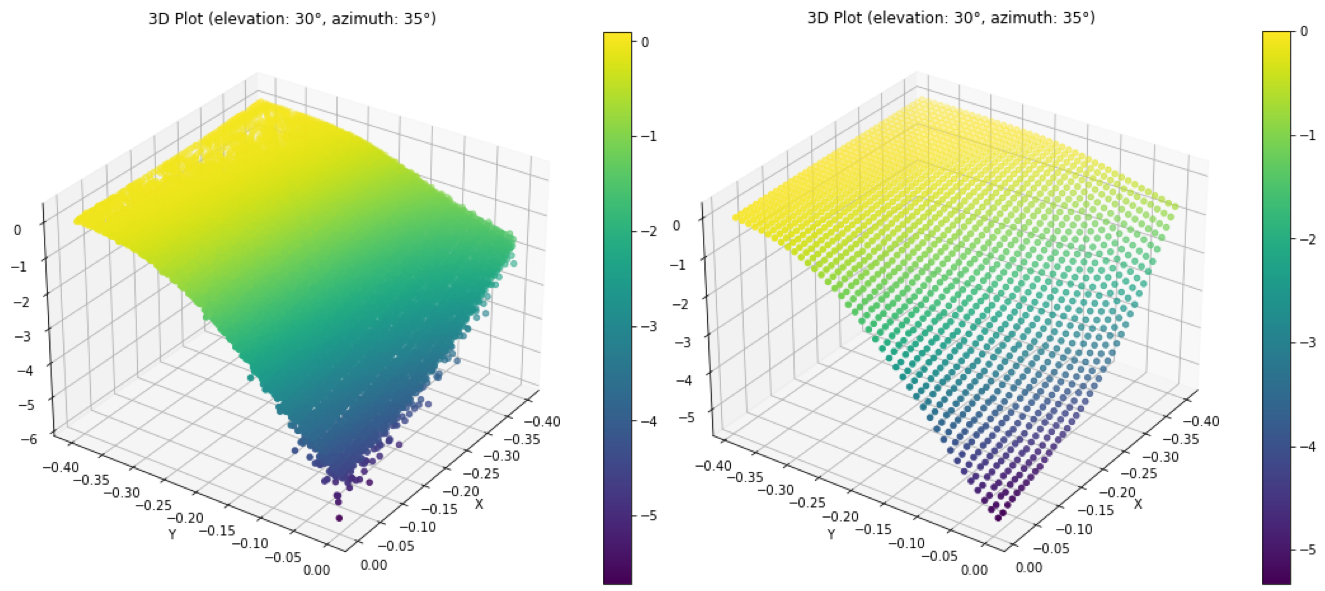
\includegraphics[width=12cm]{Fig_I_Vg}
\parbox{13cm}{\vspace*{0.5cm}
\caption{(Left) k-NN program-created results. The number of data points are 200 by
200. (Right) The number of experimentally measured data points are 40 by 40. 
The number of data points in the left-hand panel is almost three times greater than the number of data points in the right-hand panel. However, the time taken is approximately 60 minutes for both.}
\label{plot1}}
\end{figure}

\renewcommand{\figurename}{Fig. }
\begin{figure}[b]
\centering
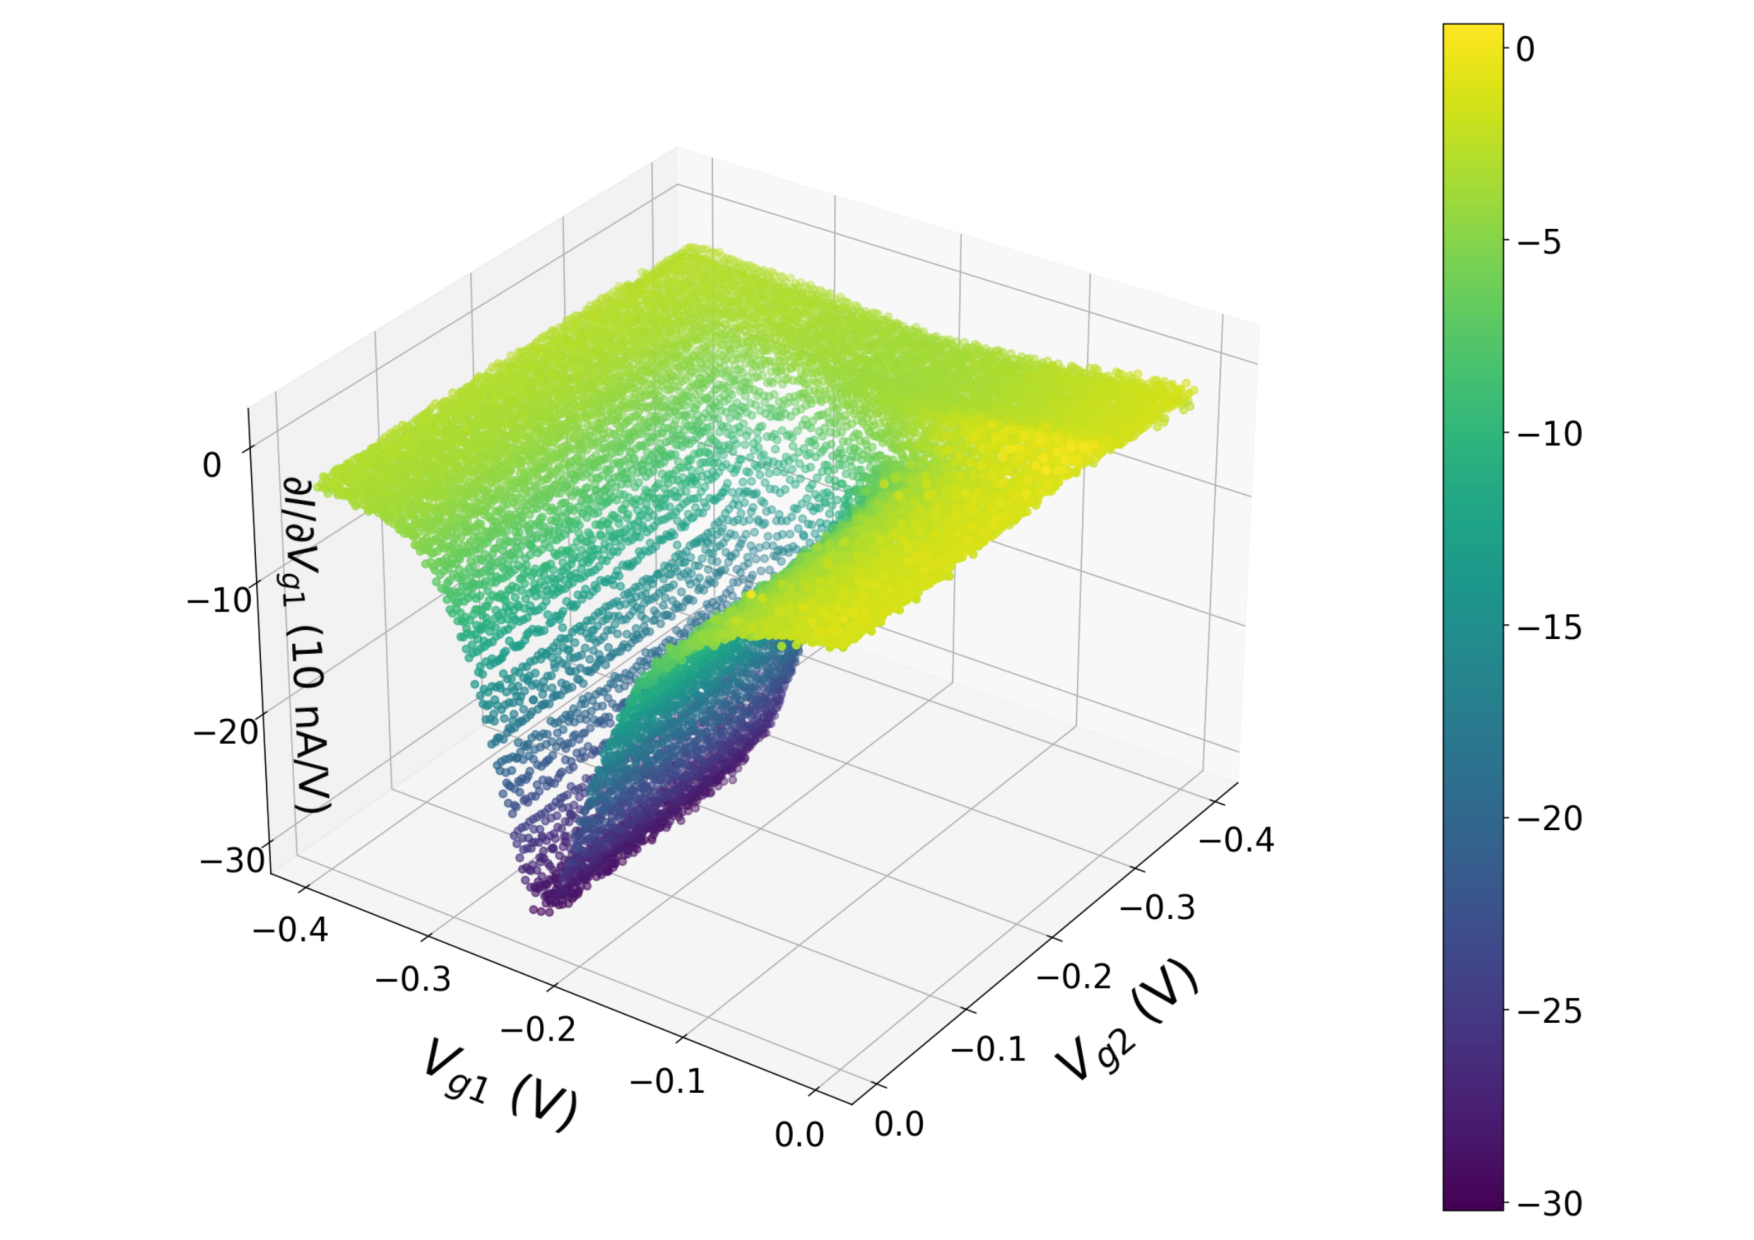
\includegraphics[width=12cm]{Fig_didv}
\parbox{13cm}{\vspace*{0.5cm}
\caption{k-NN program-created $\partial I/\partial V_{g1}$ results. The number of data points are 200 by
200. }
\label{plot1}}
\end{figure}



\begin{thebibliography}{99}
\section*{References}

\bibitem{schoinas}
Schoinas, N., Rath, Y., Norimoto, S., Xie, W., See, P., Griffiths, J.P., Chen, C., Ritchie, D.A., Kataoka, M., Rossi, A. and Rungger, I., 2024. Fast characterization of multiplexed single-electron pumps with machine learning. arXiv preprint arXiv:2405.20946.


\bibitem{bae}
Bae, M.H., Ahn, Y.H., Seo, M., Chung, Y., Fletcher, J.D., Giblin, S.P., Kataoka, M. and Kim, N., 2015. Precision measurement of a potential-profile tunable single-electron pump. Metrologia, 52(2), p.195.


\bibitem{ampere}
https://www.bipm.org/en/si-base-units/ampere;
The ampere, symbol A, is the SI unit of electric current. It is defined by taking the fixed numerical value of the elementary charge e to be $1.602 176 634 \times 10^{–19}$ when expressed in the unit C, which is equal to A s, where the second is defined in terms of $\Delta \nu _{Cs}$.

\bibitem{stein}
Stein, F., Drung, D., Fricke, L., Scherer, H., Hohls, F., Leicht, C., Götz, M., Krause, C., Behr, R., Pesel, E. and Pierz, K., 2015. Validation of a quantized-current source with 0.2 ppm uncertainty. Applied Physics Letters, 107(10).

\bibitem{pyvisa}
https://pyvisa.readthedocs.io/en/latest/





\end{thebibliography}



\end{document}




